\begin{figure}[ht]
    \centering
    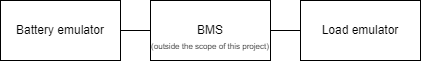
\includegraphics[scale=0.7]{Global_project_description.png}
    \caption{Hardware system that presents the BMS with a "battery" and a "load"}
    \label{fig:global_project_description}
\end{figure}

The goal of this project is to design a programmable hardware system that presents a BMS with a "battery" and a "load". The hardware system emulates the battery and load. By using only software changes the hardware system should be able to emulate a battery with a different chemistry, capacity and cell topology. Likewise the hardware system should be able to emulate different loads from electronics through to motors under varying load.

% The goal of this project is to design a programmable hardware system that presents the BMS with a “battery” and a “load.” The hardware system should, in the first iteration, be able to emulate a battery with a specific lithium-ion chemistry and capacity. However, the hardware should be flexible enough to require only software changes to emulate a battery with a different chemistry, a different capacity, and a different cell topology.

% Likewise, it should be possible to emulate different loads: from electronics through to motors under varying load.

The main deliverables are:
\begin{itemize}
    \item Tested prototype of a battery emulator circuit
    \item Research report on existing hardware emulators, and the requirements for future emulators
\end{itemize}

To be able to accomplish these deliverables it is necessary to research the following topics:
\begin{itemize}
    \item What different battery chemistries are there?
    \item How do different battery chemistries behave?
    \item What different battery cell topologies are there?
    \item How do different battery cell topologies behave?
    \item How do different battery capacities behave?
    \item What kind of loads are there?
    \item How do different loads behave?
    \item How to control the voltage, current and phase to emulate a battery cell via software changes?
    \item How to control the voltage, current and phase to emulate a load via software changes?
    \item What hardware emulators already exist?
    \item What are the future emulator requirements?
\end{itemize}

\newpage
\section{Requirements}
\begin{longtable}{|c|p{10cm}|c|c|}
    \hline
    \textbf{ID} & \textbf{Requirement} & \textbf{Priority} & \textbf{Status}\\ \hline 
    \textbf{U1} & The hardware is able to emulate a battery with a specific lithium-ion chemistry and capacity & Must & Proposed\\ \hline
    \textbf{U2} & The hardware is flexible enough to require only software changes to emulate a battery with a different chemistry, a different capacity, and a different cell topology & Must & Proposed\\ \hline
    \textbf{U3} & It is possible to emulate different loads: from electronics through to motors under varying load & Must & Proposed\\ \hline
    \textbf{U4} & The battery emulator circuit is tested & Must & Proposed\\ \hline
    \textbf{U5} & The hardware is able to control the voltage, current and phase independently & Must & Proposed\\ \hline
    \textbf{U6} & The hardware contains a BMS & Won't & Proposed\\ \hline
\end{longtable}